% !TEX root = ../../tcc.tex

\chapter[Ecossistema CEDIS]{Ecossistema CEDIS}
\label{cap:ecossistema}

O Centro de Estudo, Desenvolvimento e Inovação em Software (CEDIS) da
Universidade de Brasília (UnB) mantém um conjunto de produtos de
software integrados, voltados ao apoio do ensino e da aprendizagem em sala
de aula. Esses produtos compartilham uma mesma
base de identidade, comunicação e princípios de privacidade, formando um
ecossistema no qual o conteúdo produzido por um docente é reaproveitado,
enriquecido e observado por diferentes serviços ao longo de toda a jornada
pedagógica. A caracterização dos produtos que compõem o Ecossistema CEDIS e
o levantamento técnico detalhado da arquitetura de dados, do modelo de
dados, da taxonomia de eventos e dos mecanismos de privacidade implementados
no CEDIS Deck Manager fundamentam a compreensão dos dados de múltiplas
fontes utilizados na abordagem de \textit{Knowledge Tracing} proposta neste
trabalho.


\section{Produtos do Ecossistema}
\label{sec:produtos-ecossistema}

O Ecossistema CEDIS é composto por seis produtos integrados: CEDIS Deck
Manager, CEDIS Slides, Concept Studio + Questionários, Atlas do Conhecimento, CEDIS Learning Passport e CEDIS
Learning Analytics. Esses produtos são projetados para operar em conjunto ao longo de um
mesmo fluxo pedagógico: do planejamento do conteúdo pelo docente até a
geração de indicadores acionáveis sobre a aprendizagem dos estudantes. A
Figura~\ref{fig:ecossistema-cedis} ilustra esse panorama, evidenciando os
seis produtos e suas respectivas funcionalidades.

\begin{figure}[htb]
\caption{Panorama do Ecossistema CEDIS}
\label{fig:ecossistema-cedis}
\centering
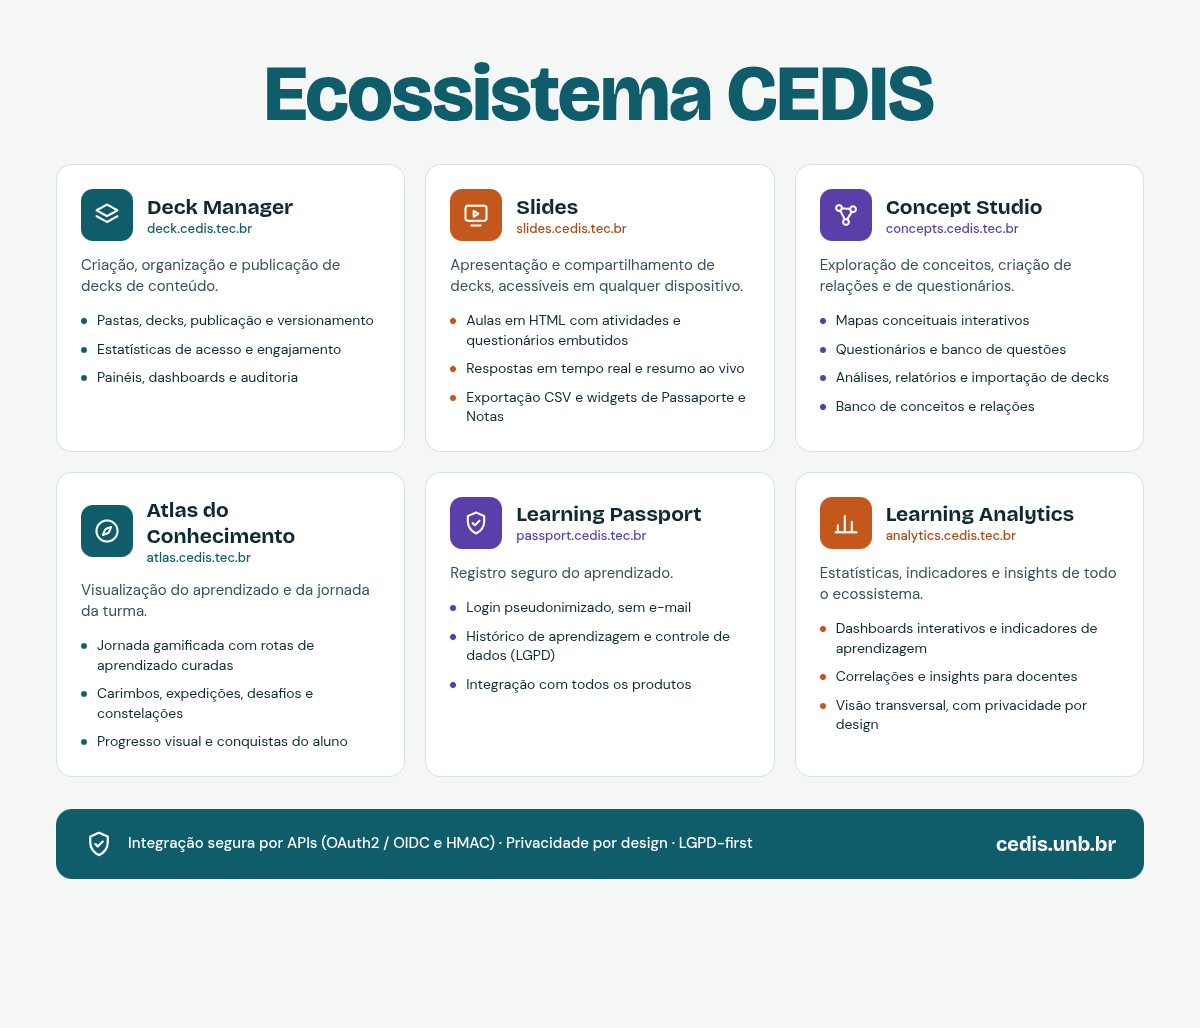
\includegraphics[width=\textwidth]{figuras/panoramaCEDIS.png}
\legend{Fonte: CEDIS/UnB.}
\end{figure}

A integração entre os produtos é realizada por meio de APIs seguras,
utilizando protocolos padronizados de autenticação e autorização (OAuth2 e
OIDC) e assinatura de mensagens (HMAC), e é orientada pelos princípios de
privacidade desde a concepção (\textit{privacy by design}) e de
conformidade com a Lei Geral de Proteção de Dados (LGPD), doravante
referidos como \textit{LGPD-first}. Essa combinação permite que dados
produzidos em um serviço sejam referenciados de forma consistente por outro
serviço sem que dados pessoais desnecessários trafeguem entre os componentes.

\subsection{CEDIS Deck Manager}
\label{subsec:deck-manager}

O CEDIS Deck Manager\footnote{Disponível em \url{https://deck.cedis.tec.br}} é o produto
responsável pelo plano operacional do ecossistema: nele o docente cria,
organiza e publica os \textit{decks} de conteúdo que serão posteriormente
apresentados em sala de aula. O produto oferece exploração e gerenciamento
de pastas e \textit{decks}, publicação com controle de versionamento,
estatísticas de acesso e engajamento por material publicado, um FAQ do
conteúdo do \textit{deck}, perfil e avatar do docente, um painel com
visões e \textit{dashboards} de uso, e um mecanismo de auditoria completa
das ações realizadas sobre o conteúdo. Por concentrar o cadastro de
usuários, a hierarquia de pastas e \textit{decks} e a telemetria de acesso
e interação, o Deck Manager funciona como o núcleo a partir do qual os
demais produtos do ecossistema obtêm contexto (por exemplo, a qual
\textit{deck} e a qual docente pertence uma determinada atividade).

\subsection{CEDIS Slides}
\label{subsec:slides}

O CEDIS Slides\footnote{Disponível em \url{https://slides.cedis.tec.br}} é o produto voltado à
apresentação dos \textit{decks} publicados pelo Deck Manager, sendo o
ponto de contato direto entre o conteúdo produzido pelo docente e o estudante
durante a aula. Ele permite apresentar e compartilhar \textit{decks} em
formato HTML acessível em qualquer dispositivo, incorporar atividades
interativas embutidas ao longo da apresentação, coletar respostas dos
estudantes em tempo real, exibir um resumo ao vivo da participação nas atividades,
exportar os dados coletados (por exemplo, em formato CSV). É neste
produto que se origina grande parte dos dados de resposta a atividades
que alimentam, posteriormente, o CEDIS Learning Analytics.

\subsection{Concept Studio + Questionários}
\label{subsec:concept-studio}

O Concept Studio\footnote{Disponível em \url{https://concepts.cedis.tec.br}} é o produto
responsável pela estruturação do conhecimento em mapas conceituais.
O módulo de questionários foi incorporado ao Concept Studio, que 
atualmente concentra a criação de mapas conceituais interativos, a
manutenção de um banco de conceitos, a criação de questionários vinculados
a esses conceitos, a geração de análises e relatórios, e a importação de
\textit{decks} já publicados no Deck Manager para vinculação a conceitos.
Esse vínculo entre atividade e conceito é um dos elementos centrais para a
abordagem de \textit{Knowledge Tracing} proposta neste trabalho, pois é o
que permite associar uma resposta de estudante a um conceito específico do domínio
de conhecimento.

\subsection{Atlas do Conhecimento}
\label{subsec:atlas}

O Atlas do Conhecimento\footnote{Disponível em \url{https://atlas.cedis.tec.br}} é o produto
voltado à experiência do estudante na exploração do conhecimento estruturado
pelo Concept Studio. Ele oferece mapas conceituais interativos, rotas de
aprendizado curadas por conceito, um sistema de emblemas e desafios e a visualização do
progresso do estudante ao longo de sua jornada.

\subsection{CEDIS Learning Passport}
\label{subsec:learning-passport}

O CEDIS Learning Passport\footnote{Disponível em \url{https://passport.cedis.tec.br}} é o
produto responsável pela identidade e pelo contexto do estudante dentro do
ecossistema. Ele oferece login sem necessidade de e-mail ou senha, um
passaporte anônimo (gerando automaticamente uma credencial única) e persistente
ao longo do percurso do estudante, um histórico consolidado de aprendizagem, e controle do estudante sobre
seus próprios dados em conformidade com a LGPD. No modelo de dados
do Deck Manager, a integração com o Learning Passport é representada pela
entidade \textit{LearningAnalyticsIngestLink}, que permite associar,
apenas quando o estudante opta explicitamente por isso, um evento de
aprendizagem a uma pessoa, grupo ou contexto identificável.

\subsection{CEDIS Learning Analytics}
\label{subsec:learning-analytics}

O CEDIS Learning Analytics\footnote{Disponível em \url{https://analytics.cedis.tec.br}} é o
produto responsável por consolidar os sinais gerados pelos demais
componentes do ecossistema em estatísticas, \textit{dashboards},
indicadores, correlações e \textit{insights} acionáveis para docentes.
Atualmente, suas análises são descritivas: no nível dos conceitos, por
exemplo, o produto contabiliza as questões respondidas correta e
incorretamente, sem inferir o domínio dos estudantes.
Ele tem caráter transversal ao ecossistema e é construído sobre os mesmos
princípios de privacidade por desenho e conformidade com a LGPD adotados
pelos demais produtos. É neste produto que os dados operacionais do Deck
Manager, as respostas do Slides, os conceitos e os questionários do Concept
Studio + Questionários e o contexto do Learning Passport convergem para
análises agregadas, e é também o produto mais diretamente relacionado ao
objetivo deste trabalho: agregar dados de múltiplas fontes do ecossistema
para fundamentar a estimativa do domínio de conceitos com \textit{Knowledge
Tracing}.

\bigskip

A Figura~\ref{fig:fluxo-interacao-cedis} resume a integração entre os seis
produtos. O docente organiza o conteúdo no Deck Manager, estrutura os
conceitos e os questionários no Concept Studio e apresenta a aula pelo
CEDIS Slides. O estudante responde às atividades em sala, responde aos
questionários no Concept Studio + Questionários e explora os conceitos no
Atlas do Conhecimento, e a sua
aprendizagem é registrada, sob o seu controle, no Learning Passport. Por
fim, os registros do ecossistema são consolidados no Learning Analytics,
que apoia as decisões pedagógicas do docente.

\begin{figure}[htb]
\caption{Fluxo de interação entre os produtos do Ecossistema CEDIS}
\label{fig:fluxo-interacao-cedis}
\centering
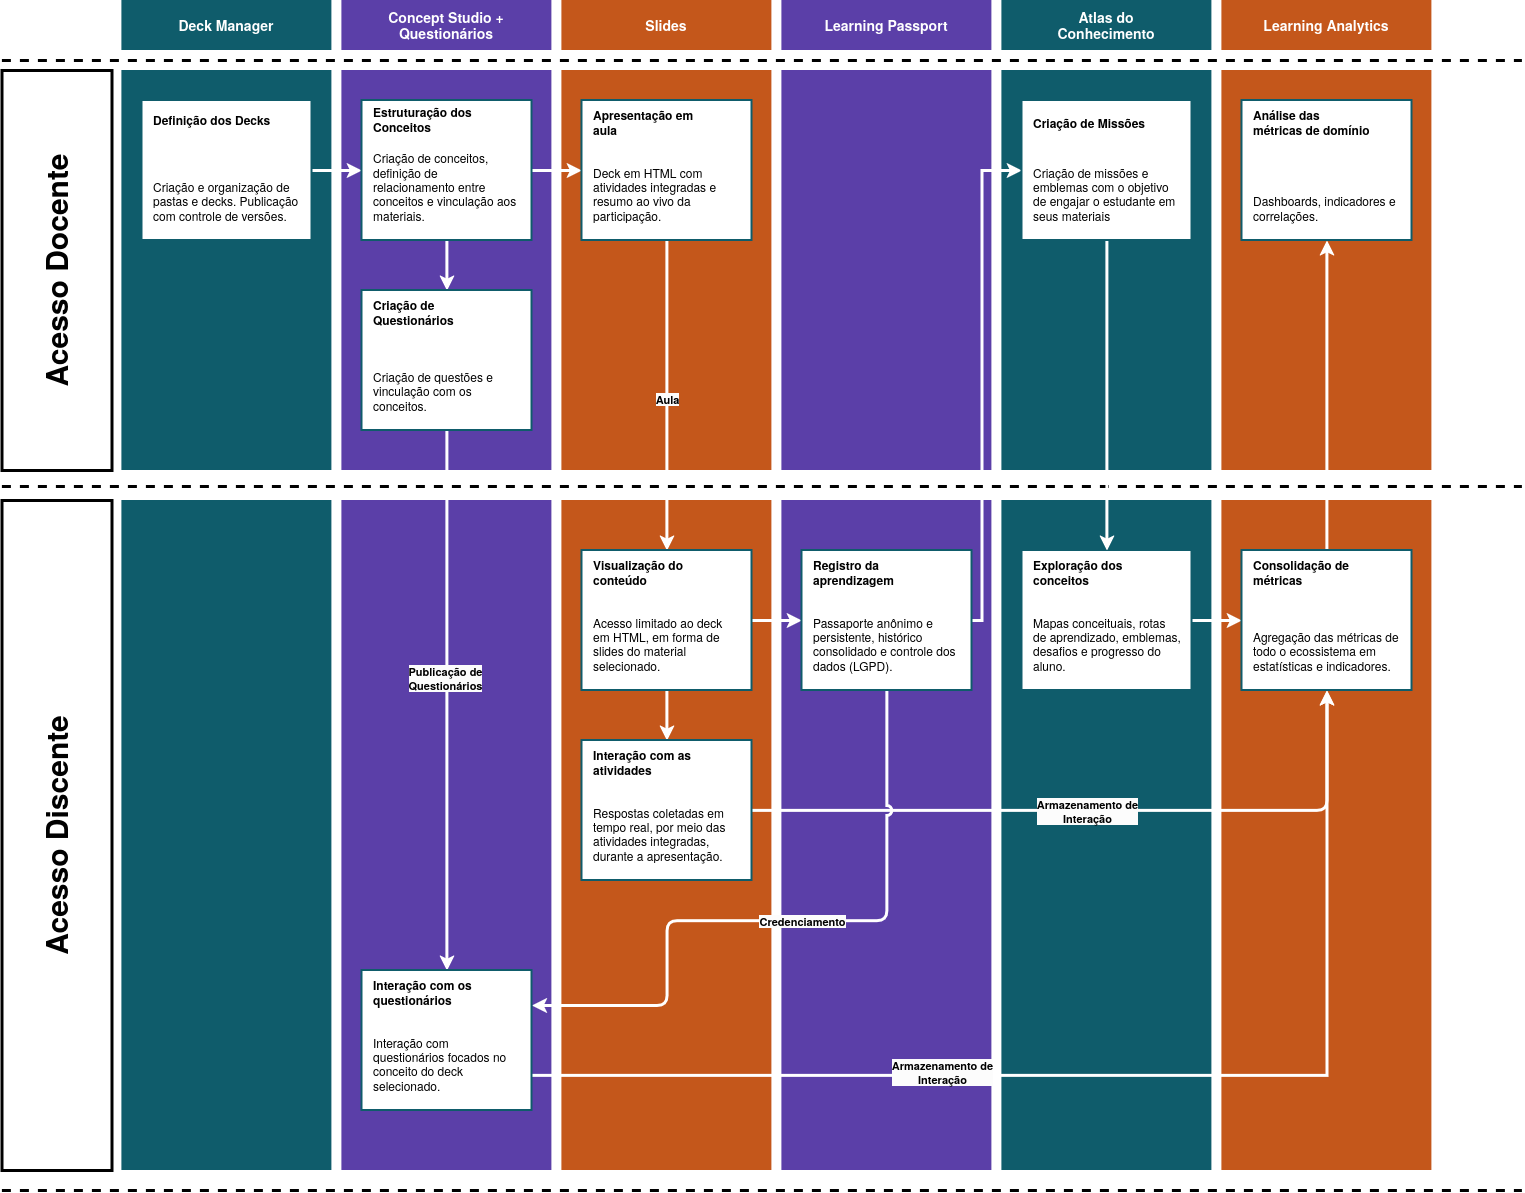
\includegraphics[width=\textwidth]{figuras/fluxo.png}
\legend{Fonte: Elaborado pelos autores.}
\end{figure}

\section{Dados Coletados do Sistema}
\label{sec:dados-coletados}

Com base em um levantamento técnico realizado sobre o
código-fonte do repositório do CEDIS Deck Manager\footnote{Levantamento
realizado sobre o repositório \texttt{cedis-unb/CEDIS-Deck-Manager}, ramo
\texttt{main}, \textit{commit} \texttt{3bb454ae885aaeef6c3950c98786acc41eda073f},
em 12 de setembro de 2026. Como critério de verdade, adotou-se o código
efetivamente implementado, tratando a documentação do repositório como
evidência secundária.}, caracterizam-se a arquitetura de dados, o modelo de dados, a
taxonomia de eventos e os mecanismos de privacidade atualmente em operação
no ecossistema. O Deck Manager foi escolhido como objeto desse
levantamento por concentrar o cadastro de usuários, o conteúdo publicado e
a telemetria de acesso e interação, além de já apresentar vínculos
explícitos, em seu modelo de dados, com os demais componentes do
ecossistema (respostas de atividades, eventos de \textit{Learning
Analytics}, banco de questões e identidade opcional).

\subsection{Arquitetura de Dados e Componentes}
\label{subsec:arquitetura-dados}

O sistema deixou de ser uma simples dupla composta por um gerenciador de
conteúdo e uma API de respostas, evoluindo para uma plataforma distribuída
com responsabilidades bem definidas por componente. O Deck Manager atua
como plano operacional e administrativo, concentrando \textit{decks}, usuários,
pastas, versões, eventos, acessos, avaliações (\textit{ratings}),
retroalimentação (\textit{feedback}) e vínculos com a camada de
\textit{Learning Analytics}. A camada pública de respostas às atividades
(\textit{cedis-slides-api}) mantém as respostas dos estudantes, a sessão e o
identificador do participante, que pode ser anônimo ou identificado, conforme
o modo configurado. A camada de ingestão de \textit{Learning Analytics}
(\textit{cedis-la-ingest}) recebe eventos padronizados de aprendizagem e
seus vínculos com respostas e identidade. O serviço de identidade
(\textit{cedis-identity-suite}) mantém dados de pessoa, grupo e contexto
apenas quando o estudante opta por habilitá-los. O serviço \textit{cedis-atlas}, que atende
ao Atlas do Conhecimento e ao Concept Studio + Questionários, mantém os
conceitos e as questões criadas no Concept Studio + Questionários. Por
fim, o pacote \textit{cedis-core}, externo ao repositório do Deck Manager,
fornece contratos e modelos de conteúdo compartilhados entre os
componentes. A Tabela~\ref{tab:componentes-cedis} resume o papel, os
principais dados e a forma de persistência e consumo de cada componente.

\begin{table}[htb]
\caption{Componentes de dados do ecossistema e seus papéis}
\label{tab:componentes-cedis}
\centering
\begin{tabularx}{\textwidth}{l>{\raggedright\arraybackslash}X>{\raggedright\arraybackslash}X}
\hline
\textbf{Componente} & \textbf{Papel} & \textbf{Dados principais} \\
\hline
Navegador / apresentação & Produtor primário de eventos & Eventos de navegação, atividade, respostas e contexto de sessão \\
\hline
Deck Manager & Plano operacional e analítico & \textit{Decks}, usuários, pastas, versões, eventos, acessos, avaliações, \textit{feedback}, vínculos com \textit{Learning Analytics} \\
\hline
CEDIS Slides (\textit{slides-api}) & Plano público de resposta & Respostas de atividades, sessão, participante anônimo ou identificado, conteúdo da resposta \\
\hline
\textit{LA Ingest} & Ingestão de \textit{Learning Analytics} & Eventos de aprendizagem padronizados e seus vínculos \\
\hline
\textit{Identity Suite} (Learning Passport) & Identidade e contexto opcional & Pessoa, grupo e contexto, apenas quando habilitados pelo estudante \\
\hline
\textit{cedis-atlas} & Conceitos e questões (Atlas do Conhecimento e Concept Studio + Questionários) & Mapas conceituais, conceitos e questões vinculadas às atividades \\
\hline
\textit{cedis-core} & Modelos compartilhados & Contratos e modelos de conteúdo de versão/\textit{commit} compartilhados (dependência externa) \\
\hline
\end{tabularx}
\legend{Fonte: Elaborado pelos autores a partir de levantamento técnico do repositório CEDIS Deck Manager (\textit{commit} \texttt{3bb454a}, 2026).}
\end{table}

Dentro dessa arquitetura, coexistem trilhas de dados com finalidades
distintas: telemetria operacional de acesso e navegação, respostas
educacionais às atividades, eventos padronizados de \textit{Learning
Analytics} e, opcionalmente, dados de identidade. Essas trilhas não devem
ser tratadas como equivalentes entre si, pois cada uma possui semântica,
política de retenção e nível de sensibilidade próprios. Essa distinção tem
implicações diretas para a forma como dados de múltiplas fontes podem ser
combinados de maneira íntegra e reprodutível em uma abordagem de
\textit{Knowledge Tracing}.

\subsection{Modelo de Dados}
\label{subsec:modelo-dados}

O núcleo do Deck Manager é composto por entidades de conteúdo, usuários,
acesso e telemetria, versionamento de conteúdo, avaliação e
retroalimentação, mapeamento de questões e vínculo com a camada de
\textit{Learning Analytics}. A Tabela~\ref{tab:entidades-deck-manager}
apresenta as entidades centrais confirmadas no código-fonte do
componente, com sua chave de identificação, seus principais
relacionamentos e os campos mais relevantes para fins analíticos e de
privacidade.

\begin{table}[htb]
\caption{Entidades centrais do modelo de dados do CEDIS Deck Manager}
\label{tab:entidades-deck-manager}
\centering
\begin{tabularx}{\textwidth}{l>{\raggedright\arraybackslash}X>{\raggedright\arraybackslash}X}
\hline
\textbf{Entidade} & \textbf{Relacionamentos} & \textbf{Campos analíticos e de privacidade} \\
\hline
\textit{User} & Proprietário de avaliações, \textit{feedback} e eventos quando autenticado & Perfil (\textit{role}), estado da conta, consentimentos, último acesso \\
\hline
\textit{Folder} & Auto-relacionamento (hierarquia); contém \textit{decks} & Identificador do proprietário, data de criação e atualização \\
\hline
\textit{Deck} & Pertence a uma pasta; possui versões, marcações e eventos & Status, data de publicação, versão, configurações, \textit{checksum} \\
\hline
\textit{ContentVersion} & Um \textit{deck} possui várias versões & Número da versão, data de criação, \textit{checksum}, URL do pacote \\
\hline
\textit{DeckAccess} & Associado a um \textit{deck}; usuário opcional & Sessão, \textit{hash} do IP de origem, agente do usuário, data e hora do acesso \\
\hline
\textit{DeckEvent} & Associado a um \textit{deck}; usuário opcional & Tipo do evento, atividade, código de sessão, identificador anônimo de visitante, classe de dispositivo e de origem, metadados \\
\hline
\textit{QuestionActivityMap} & Vincula um \textit{deck}/atividade a uma questão externa (\textit{cedis-atlas}) & Identificador da atividade, identificador da questão, data de criação \\
\hline
\textit{LearningAnalyticsIngestLink} & Vincula um evento de \textit{Learning Analytics} a uma resposta e, opcionalmente, a uma identidade & Identificador do evento de ingestão, identificadores de pessoa/grupo/contexto, metadados \\
\hline
\textit{DeckRating} & Um único \textit{rating} por par usuário/\textit{deck} & Número de estrelas, comentário, data de criação \\
\hline
\textit{Feedback} & Associado a um \textit{deck}; usuário opcional & \textit{Hash} do IP de origem, agente do usuário, sinalização de anonimização \\
\hline
\end{tabularx}
\legend{Fonte: Elaborado pelos autores a partir de levantamento técnico do repositório CEDIS Deck Manager (\textit{commit} \texttt{3bb454a}, 2026).}
\end{table}

Do ponto de vista do objetivo deste trabalho, duas entidades merecem
destaque. A primeira é \textit{QuestionActivityMap}, que estabelece o
vínculo entre uma atividade de um \textit{deck} e uma questão do banco de
questões do \textit{cedis-atlas}, permitindo associar respostas a conceitos
específicos, o que é pré-requisito para qualquer modelagem de \textit{Knowledge
Tracing}. A segunda é \textit{LearningAnalyticsIngestLink}, que formaliza
a reconciliação entre um evento padronizado de aprendizagem, uma resposta
persistida e, opcionalmente, uma identidade, constituindo o ponto de
integração de dados de múltiplas fontes do ecossistema em um único
registro analítico. Cabe ressaltar que essas referências entre serviços
são lógicas, e não chaves estrangeiras físicas de um mesmo banco de
dados: a integridade referencial entre \textit{QuestionActivityMap},
\textit{LearningAnalyticsIngestLink} e as respostas mantidas pelo CEDIS
Slides depende de contratos de API, validação e mecanismos de
reconciliação, e não apenas de restrições do banco de dados relacional do
Deck Manager.

\subsection{Taxonomia de Eventos de Interação}
\label{subsec:taxonomia-eventos}

A camada de \textit{analytics} do Deck Manager valida explicitamente cinco
tipos de evento de interação; eventos fora desse conjunto são rejeitados
ou ignorados, o que garante uma taxonomia mínima estável para fins de
análise. A Tabela~\ref{tab:eventos-deck-manager} descreve a semântica
operacional de cada evento e as principais métricas que podem ser
derivadas a partir dele.

\begin{table}[htb]
\caption{Taxonomia de eventos de interação do CEDIS Deck Manager}
\label{tab:eventos-deck-manager}
\centering
\begin{tabularx}{\textwidth}{l>{\raggedright\arraybackslash}X>{\raggedright\arraybackslash}X}
\hline
\textbf{Evento} & \textbf{Semântica operacional} & \textbf{Métricas deriváveis} \\
\hline
\textit{deck\_open} & \textit{Deck} acessado/aberto & Número de aberturas, visitantes por dia, origem e dispositivo \\
\hline
\textit{activity\_impression} & Atividade apresentada/visível ao estudante & Número de impressões, alcance da atividade \\
\hline
\textit{activity\_started} & Início explícito da atividade pelo estudante & Taxa de início, abandono anterior à submissão \\
\hline
\textit{activity\_submitted} & Submissão da atividade registrada como evento & Taxa de submissão, funil de participação \\
\hline
\textit{summary\_view} & Resumo da atividade visualizado & Taxa de visualização do resumo \\
\hline
\end{tabularx}
\legend{Fonte: Elaborado pelos autores a partir de levantamento técnico do repositório CEDIS Deck Manager (\textit{commit} \texttt{3bb454a}, 2026).}
\end{table}

Esses cinco eventos formam o funil operacional \textit{deck\_open}
$\rightarrow$ \textit{activity\_impression} $\rightarrow$
\textit{activity\_started} $\rightarrow$ \textit{activity\_submitted}
$\rightarrow$ \textit{summary\_view}, que descreve a jornada de um estudante
dentro de uma única atividade. Duas limitações desses dados devem
ser destacadas. Primeiro, o evento \textit{activity\_submitted} é
registrado independentemente da resposta persistida em
\textit{activity\_responses}, e os dois registros podem divergir em caso
de falha parcial de envio. Segundo, como o identificador anônimo de
visitante é recalculado diariamente, a telemetria anônima não permite
reconstruir a trajetória de um mesmo estudante ao longo de dias distintos.

\subsection{Privacidade, Anonimização e Conformidade com a LGPD}
\label{subsec:privacidade}

O Deck Manager implementa mecanismos de privacidade desde a concepção,
principalmente na telemetria de interação. O visitante é identificado por
um código pseudonimizado (\textit{anon\_visitor\_hash}), gerado por
HMAC-SHA256 com rotação diária a partir de atributos minimizados, como o
prefixo de rede do endereço IP e as classes de idioma e de dispositivo, sem
armazenar o endereço IP completo ou o agente de usuário bruto. Além disso, o
sistema respeita o sinalizador \textit{Do Not Track} (DNT), filtra o
tráfego automatizado (\textit{bots}) e aplica \textit{k}-anonimato aos
relatórios agregados. Como o identificador muda a cada dia, essa telemetria
não permite acompanhar um mesmo estudante ao longo do tempo, o que só é
possível por meio da identidade consentida no Learning Passport. A
Tabela~\ref{tab:privacidade-deck-manager} resume esses mecanismos e seu
efeito sobre a análise dos dados.

\begin{table}[htb]
\caption{Mecanismos de privacidade e anonimização do CEDIS Deck Manager}
\label{tab:privacidade-deck-manager}
\centering
\begin{tabularx}{\textwidth}{l>{\raggedright\arraybackslash}X>{\raggedright\arraybackslash}X}
\hline
\textbf{Mecanismo} & \textbf{Efeito analítico} & \textbf{Governança necessária} \\
\hline
\textit{Hash} diário (HMAC) & Impede rastreamento longitudinal estável de um mesmo visitante & Chave secreta, rotação periódica, vedação à tentativa de reidentificação \\
\hline
Prefixo de IP (/24 ou /48) & Reduz a precisão de geolocalização e pode colidir sob NAT & Não deve ser tratado como identidade de pessoa ou dispositivo \\
\hline
Classificação de agente de usuário & Permite segmentação por classe de dispositivo sem armazenar o agente bruto & Tabelas que ainda armazenam o agente bruto (\textit{DeckAccess}, \textit{Feedback}) exigem política própria \\
\hline
\textit{Do Not Track} (DNT) & Gera ausência voluntária de dados (\textit{missingness}) & Métricas devem reconhecer cobertura incompleta, sem imputação como ausência de uso \\
\hline
Filtragem de \textit{bots} & Melhora a qualidade do tráfego considerado humano & Regras devem ser mantidas testadas e versionadas \\
\hline
\textit{k}-anonimato & Suprime células pequenas em relatórios agregados & Exibir indicador de supressão em vez de valor zero \\
\hline
Identidade opcional (\textit{opt-in}) & Habilita contexto individual apenas quando legítimo e consentido & Exige base legal, finalidade explícita, minimização, controle de acesso e retenção segregados \\
\hline
\end{tabularx}
\legend{Fonte: Elaborado pelos autores a partir de levantamento técnico do repositório CEDIS Deck Manager (\textit{commit} \texttt{3bb454a}, 2026).}
\end{table}

Esses mecanismos estabelecem duas distinções importantes para este
trabalho. A primeira é que pseudonimizar não equivale a anonimizar: o
\textit{anon\_visitor\_hash}, ainda que rotativo, é um pseudônimo, e
não um dado anônimo em sentido estrito. A segunda é que a base legal que
ampara a operação da plataforma e o consentimento para fins de pesquisa
não são sinônimos: o uso de dados do ecossistema em uma pesquisa científica,
como a proposta de \textit{Knowledge Tracing} deste trabalho, deve
considerar a governança ética aplicável a pesquisas com seres humanos,
independentemente da base legal que ampara a operação da plataforma.

\subsection{Métricas Existentes}
\label{subsec:metricas-existentes}

A partir dos eventos de interação e das entidades do modelo de dados, o
Deck Manager já deriva um conjunto de métricas operacionais e
descritivas, entre as quais se destacam: número de aberturas de
\textit{deck} (\textit{deck opens}), número de visitantes distintos por
dia (\textit{visitor-days}), número de impressões de atividade, taxa de
início (\textit{starts / impressions}), taxa de submissão
(\textit{submissions / starts}), número de respostas persistidas, média de
respostas em escala Likert e média das avaliações (\textit{ratings}) de
um \textit{deck}. Essas métricas descrevem o uso e o engajamento, mas não
são evidência direta de aprendizagem. A relação entre a exposição a um
conteúdo e a resposta a uma atividade não estabelece, por si só,
causalidade pedagógica, e os próprios mecanismos de privacidade (DNT,
filtragem de \textit{bots} e \textit{k}-anonimato) introduzem ausência
intencional de dados. Por isso, este trabalho não reutiliza diretamente
essas métricas: combina as respostas às atividades e aos questionários com
o mapeamento atividade-conceito do Concept Studio + Questionários, de modo a estimar o domínio de conceitos de cada estudante por
meio do \textit{Knowledge Tracing}.
